\section{Fonctionnalités}
Les différentes fonctionnalités de {\bf Erub} sont : \\
{\bf Administratif} : commandes réservés au propriétaire/créateur du serveur
    \begin{itemize}
        \item{\bf ?purge nombre}  Permet de supprimer entre 1 et 100 messages de moins de 14 jours d'un channel
        
        \item{\bf ?eval arguments}  Cette commande permet à l'utilisateur d'effectuer n'importe quel calcul.
        ex: {\bf?eval (5*6)/2+5*((4/2)+5) = 50}
        
    \end{itemize}
    
    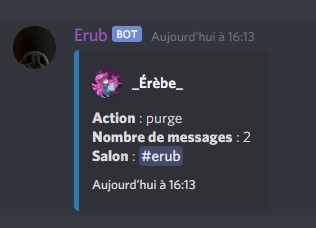
\includegraphics[width=6cm]{img/purge.jpg}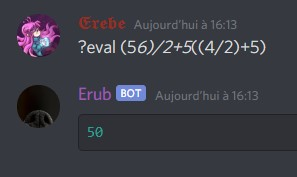
\includegraphics[width=7cm]{img/eval.jpg}
    
{\bf Jeux}: 
    \begin{itemize}
        \item {\bf ?chifumi} Permet de jouer aléatoirement donc le bot au chifoumi
        \item {\bf ?pierre} Permet de jouer pierre contre le Bot
        \item {\bf ?feuille} Permet de jouer feuille contre le Bot
        \item {\bf ?ciseaux}  Permet de jouer ciseaux contre le Bot
        \item {\bf ?pile} ou {\bf ?face} permet de lancer une pièce
        
    \end{itemize}
    
     
\includegraphics[width=6cm]{img/face2.jpg}
\includegraphics[width=7cm]{img/pile.jpg}
    \newpage
{\bf Sondages}: 
    \begin{itemize}
        \item {\bf ?poll votre question} Permet de générer un sondage avec pour réponses  oui ou non

        \item {\bf ?poll2 votre question/votre réponse 1/votre réponse 2/votre réponse 3} Permet de générer un sondage avec des arguments, vous pouvez définir jusqu'à 10 réponses qui seront numérotés de 1 à 10.
        
    \end{itemize}
    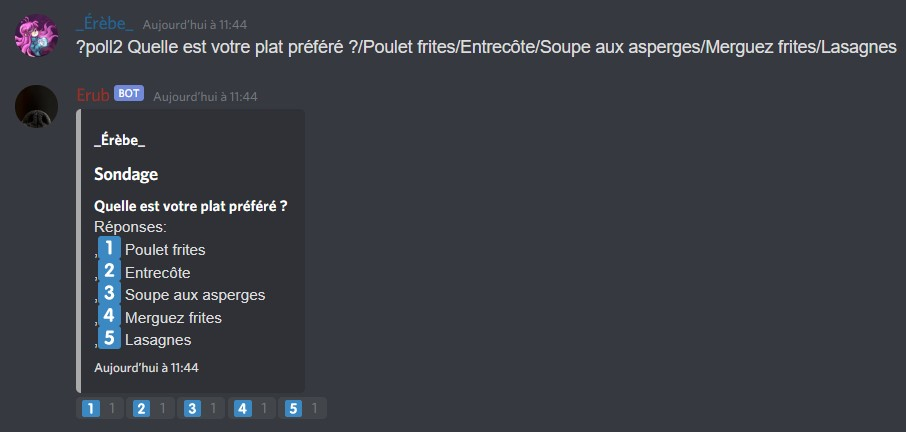
\includegraphics[width=10cm]{img/poll2.jpg} 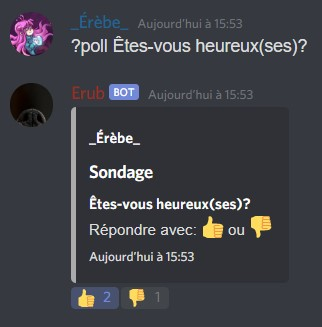
\includegraphics[width=5cm]{img/poll.jpg}
    
{\bf Informatif}: 
    \begin{itemize}
        \item{\bf ?help}  Cette commande permet à un utilisateur de demander les commandes disponibles par le bot
        
        \item {\bf ?botinfo} Permet d'afficher les informations du bot
        
        \item {\bf ?userinfo} Permet d'afficher nos informations Discord 
        
        \item {\bf ?userinfo @autre\_user} Permet d'avoir les informations d'un autre utilisateur du serveur.
        
        \item {\bf ?serverinfo} Permet d'afficher les informations du serveur

    \end{itemize}
    
    Affichage des informations utilisateurs: 
    
    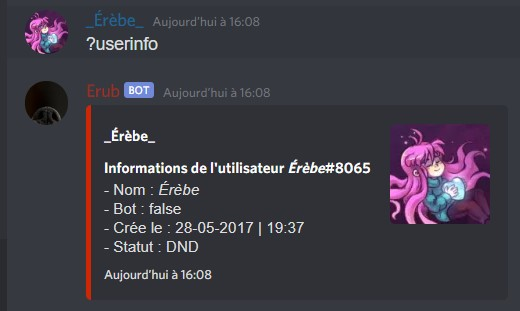
\includegraphics[width=8cm]{img/userinfo_dnd.jpg}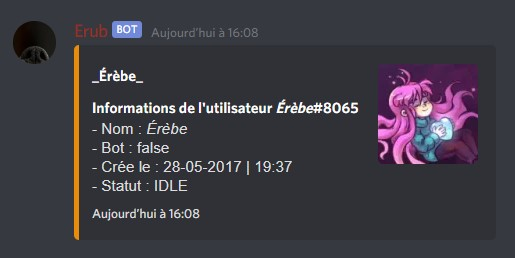
\includegraphics[width=9cm]{img/userinfo_idle.jpg}
    
    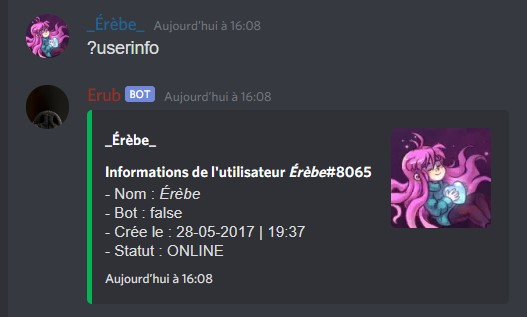
\includegraphics[width=8cm]{img/userinfo_online.jpg}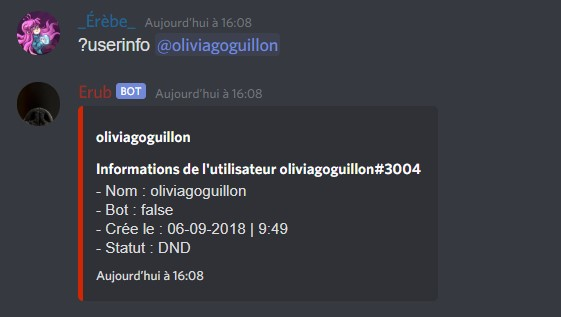
\includegraphics[width=9cm]{img/userinfo_otheruser.jpg}
    
    Commande help: 
    
    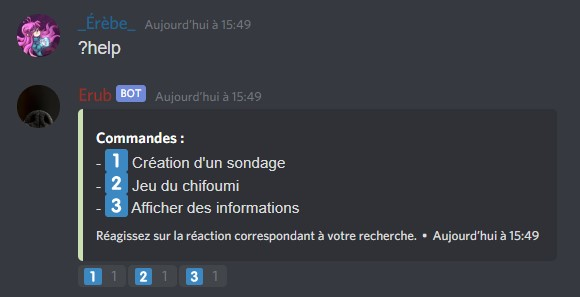
\includegraphics[width=10cm]{img/help.jpg}
    
    Informations du serveur:
    
    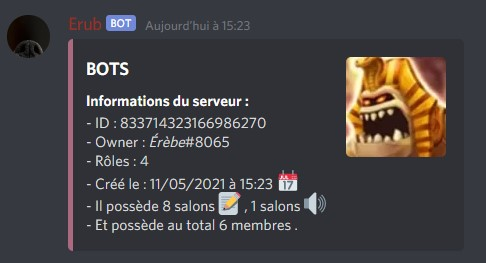
\includegraphics[width=10cm]{img/serverinfo.jpg}
    
    Informations bots, pages allant de 1 à 5: 
    
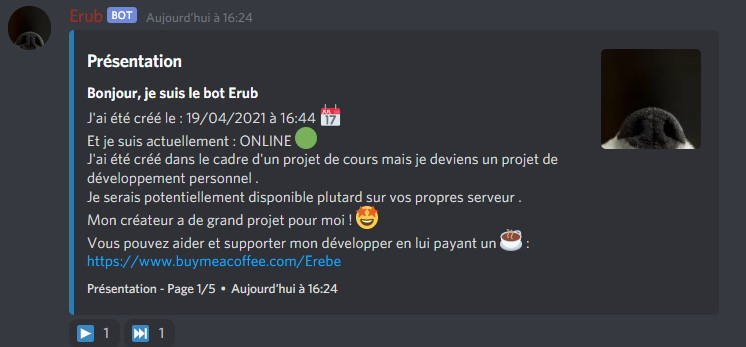
\includegraphics[width=9cm]{img/botinfo_page_1.jpg}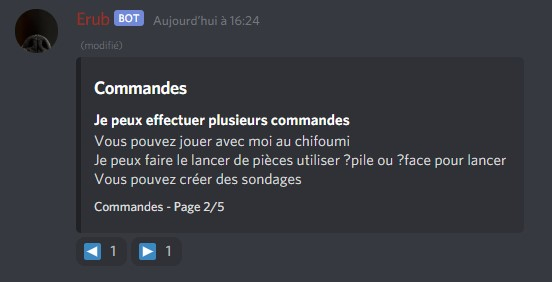
\includegraphics[width=8cm]{img/botinfo_page_2.jpg}
    
    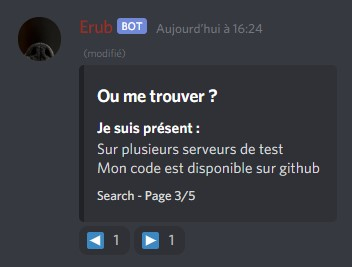
\includegraphics[width=7cm]{img/botinfo_page_3.jpg}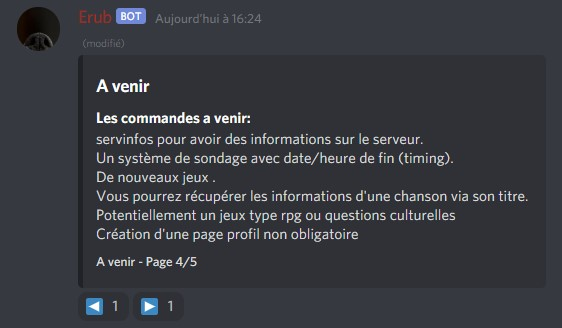
\includegraphics[width=10cm]{img/botinfo_page_4.jpg}
    
    
\includegraphics[width=12cm]{img/botinfo_page_5.jpg}